\chapter{EXPERIMENTS}
\label{Chapter4}

\section{Dataset}

\begin{figure}[H]
	\centering
	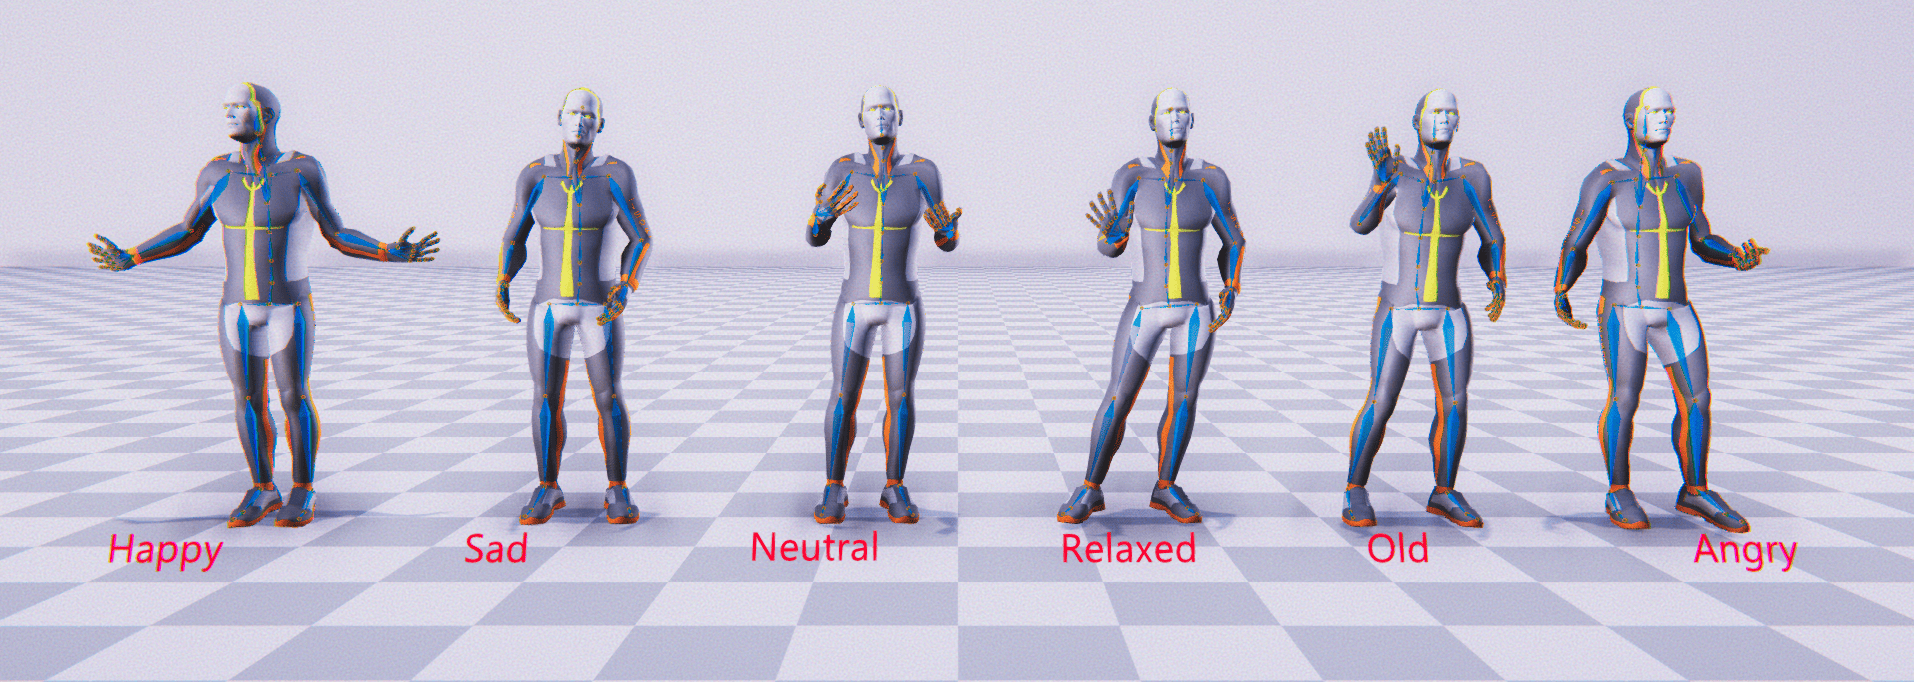
\includegraphics[width=\textwidth]{EmotionAnimation}
	\caption{Illustration of 6 gestures: $\texttt{Happy}$, $\texttt{Sad}$, $\texttt{Neutral}$, $\texttt{Old}$, $\texttt{Relaxed}$, and $\texttt{Angry}$}
\end{figure}

This thesis uses the ZeroEGGS dataset \cite{ghorbani2022zeroeggszeroshotexamplebasedgesture}, a motion capture dataset designed for research and development of gesture generation models. It includes 67 monologue clips performed by a female motion capture actor, with a total duration of 135 minutes. The monologues are annotated with 6 different emotions: $\texttt{Happy}$, $\texttt{Sad}$, $\texttt{Neutral}$, $\texttt{Old}$, $\texttt{Relaxed}$, and $\texttt{Angry}$, enabling simulation of various emotional states in gestures and body movements. ZeroEGGS provides a rich platform for studying the integration of speech and dynamic gestures, supporting the development of models capable of adapting gestures according to emotions and text semantics.

\section{Data Preprocessing}
\label{sec:Preprocessing}

In stage {1. Data Preprocessing} (\autoref{fig:CommonStage}), gesture, speech, and text data are read and processed to be represented as vectors or matrices containing information derived from raw data.

For \textbf{text data}: the thesis uses the $\texttt{nltk}$ library for tokenization and $\texttt{contractions}$ to normalize contracted words.

One contribution of the thesis is to convert the speech data available in ZeroEGGS using Adobe Speech To Text, then align the phonetic timestamps using the Montreal Forced Aligner \cite{saxon2020robust} with an English phoneme dictionary to match the gesture frame rate, generating TextGrid files. From these TextGrids containing word-level timing information, the thesis uses $\texttt{gensim}$ to generate word2vec embeddings.

\textbf{Gesture data} consists of BVH (BioVision Motion Capture) files captured via motion capture systems. BVH files include two components: Hierarchy and Motion. Specifically:

\begin{itemize}
	\item \texttt{HIERARCHY}: defines a skeletal tree containing 75 bones $\{ \mathbf{b}_1, \mathbf{b}_2 \cdots \mathbf{b}_{75} \}$, each with an initial position (\texttt{OFFSET}) and \texttt{CHANNELS} parameters specifying the type and order of rotation angles (\texttt{Zrotation}, \texttt{Yrotation}, \texttt{Xrotation}) and position (\texttt{Xposition}, \texttt{Yposition}, \texttt{Zposition}), which are defined in the \texttt{MOTION} section. The first bone (usually \texttt{Hips}) is the root bone $\mathbf{b}_{\text{root}}$, used to define the T-pose via forward kinematics as the initial pose of the skeleton before applying motion.
	
	\item \texttt{MOTION}: a sequence of frames, each containing motion data representing changes of all $75$ bones as defined by the \texttt{CHANNELS} in the \texttt{HIERARCHY}.
\end{itemize}

The model in the thesis converts Euler rotation angles to quaternion rotation angles, where a quaternion is a 4-dimensional vector.

\begin{equation} \label{eq:gesturevector}
	\mathbf{g} = \Big[ \mathbf{p}_{\text{root}},  \mathbf{r}_{\text{root}},
	\mathbf{ p }'_{\text{root}},  \mathbf{r}'_{\text{root}},
	\mathbf{p}_{\text{joins}},  \mathbf{r}_{\text{joins}},
	\mathbf{p}'_{\text{joins}},  \mathbf{r}'_{\text{joins}},
	\mathbf{d}_{\text{gaze}}
	\Big]
\end{equation}

Here, each $\mathbf{g} \in \mathbb{R}^{1141}$ includes:
{
	\begin{itemize}
		\item $\mathbf{p}_{\text{root}} \in \mathbb{R}^3$: coordinates of the root joint
		\item $\mathbf{r}_{\text{root}} \in \mathbb{R}^4$: rotation (quaternion) of the root joint
		\item $\mathbf{p}'_{\text{root}} \in \mathbb{R}^3$: velocity of the root position
		\item $\mathbf{r}'_{\text{root}} \in \mathbb{R}^3$: angular velocity of the root rotation
		
		\item $\mathbf{p}_{\text{joins}} \in \mathbb{R}^{3 n_{\text{join} }}$: positions of other joints
		\item $\mathbf{r}_{\text{joins}} \in \mathbb{R}^{6 n_{\text{join} }}$: joint rotations on the X and Y planes
		\item $\mathbf{p}'_{\text{joins}} \in \mathbb{R}^{3n_{\text{join} }}$: velocity of joint positions
		\item $\mathbf{r}'_{\text{joins}} \in \mathbb{R}^{3n_{\text{join} }}$: angular velocity of joint rotations
		\item $\mathbf{d}_{\text{gaze}} \in \mathbb{R}^3$: gaze direction
\end{itemize}}

The original gesture sequences in Euler angles are converted to radians, then converted from Euler to Quaternion as detailed in \autoref{appendix:BVHData:QuaternionConvert}.

\textbf{Speech data}: $\mathbf{a}_{\text{raw}} \in \mathbb{R}^{ \text{length } }$ is raw speech sampled at 16000 Hz, trimmed into segments $\mathbf{a} \in \mathbb{R}^{64000}$ corresponding to 4 seconds. The thesis uses \texttt{ffmpeg-normalize} to normalize volume to a level lower than the original.

\textbf{Emotion}: Emotion data is represented using a predefined one-hot encoded vector. During sampling, the filename encodes the target emotion.

All data is stored using the $\texttt{h5}$ format.

\section{Training Process}

The entire model training process was conducted over approximately two weeks with the following parameters: number of training steps $T = 1000$, using an Nvidia 3090 GPU. The learning rate was set to $3 \times 10^{-5}$, batch size was $640$, and a total of $43,853$ samples were trained. At each step, $t$ is randomly sampled and input to $f_{\theta}$ to predict $\mathbf{x}_{0}$. The emotional control parameter was set to $\gamma = 0.1$. The probability of applying random masking to the emotion and initial gesture matrices was $10\%$, using a Bernoulli distribution to randomly hide/reveal these matrices.

The $\beta$ parameter was scheduled linearly from $0.5 \rightarrow 0.999$.

The $\operatorname{HuberLoss} (\mathbf{x}_{0},  \hat{\mathbf{x}}_{0} )$ is computed as follows:

\begin{itemize}
\item If $|\mathbf{x}_0 - \hat{\mathbf{x}}_0| \leq \delta$ then $\mathcal{L}_{ \delta, \mathbf{x}_0, \hat{\mathbf{x}}_0} = \frac{1}{2} (\mathbf{x}_0 - \mathbf{x}_0)^2$: Below the threshold, the loss is computed as squared distance (similar to MSE), which is sensitive to small errors and provides smooth gradients.

\item If $|\mathbf{x}_0 - \hat{\mathbf{x}}_0| > \delta$ then $\mathcal{L}_{ \delta, \mathbf{x}_0, \hat{\mathbf{x}}_0}  =  \delta \cdot |\mathbf{x}_0 - \mathbf{x}_0| - \frac{1}{2} \delta^2$: Above the threshold, the loss behaves like MAE, reducing sensitivity to large errors and improving robustness against outliers.

\end{itemize}

The training process is implemented in the open-source repository: \hyperlink{https://github.com/hmthanh/OHGesture}{Github/OHGesture} \footnote{\url{https://github.com/hmthanh/OHGesture}}.

\section{Rendering Process in Unity}
\label{sec:Render}

To visualize the gesture generation process from model output, the thesis uses Unity in stage \textit{7. Rendering} (\autoref{fig:CommonStage}), extending code from the DeepPhase model \cite{starke2022deepphase}. The generated output is in BVH (BioVision Motion Capture) format. In Unity, the author adds C-Sharp scripts to render gestures based on coordinates and labels, with bone positions and rotations represented using quaternions.

Rendering details are presented in \autoref{Appendix3}.

The Unity project source code is available at: \hyperlink{https://github.com/DeepGesture/deepgesture-unity}{Github/DeepGesture-Unity}
\footnote{\url{https://github.com/DeepGesture/deepgesture-unity}}.
